\documentclass[11pt]{report}
\usepackage[utf8]{inputenc}
\usepackage[margin=2.0cm]{geometry}
\usepackage{fancyhdr}
\usepackage{xcolor}
\usepackage{minted}
\usepackage{graphicx}
\usepackage[parfill]{parskip}

\title{Digital Engineering\\Lab 1}
\author{Y3890959\\Y3878784}
\date{24th January 2023}

\pagestyle{fancy}
\fancyhead{}
\setlength{\headheight}{14pt}
\fancyhead[L]{Lab 1}
\fancyhead[R]{Y3890959, Y3878784}
\fancyfoot{}
\fancyfoot[L]{Digital Engineering}
\fancyfoot[R]{\thepage}

\makeatletter
\let\ps@plain\ps@fancy 
\makeatother

\setminted {
    fontsize=\footnotesize,
    frame=single,
}

\begin{document}

\maketitle

\chapter*{Task A: Debouncer implementation and simulation by parameterization}

\section*{VHDL Code}

\subsection*{Top-Level Entity}
\inputminted{vhdl}{../../Lab1/Lab1.srcs/sources_1/imports/new/fibonacci_8bit_sequence.vhd}

\subsection*{Efficient (Updated) Debouncer Entity}
\inputminted{vhdl}{../../Lab1/Lab1.srcs/sources_1/new/efficient_debouncer.vhd}

\subsection*{Counter Entity}
\inputminted{vhdl}{../../Lab1/Lab1.srcs/sources_1/new/parameterizable_counter.vhd}

\subsection*{ROM Entity}
\inputminted{vhdl}{../../Lab1/Lab1.srcs/sources_1/imports/new/fibonacci_8bit_async_read_rom.vhd}



\section*{Testbenches and Simulation}

\subsection*{Testbech VHDL Code}
\inputminted{vhdl}{../../Lab1/Lab1.srcs/sim_1/imports/new/fibonacci_8bit_sequence_tb.vhd}



\subsection*{Testbench Waveforms}

\subsubsection*{Entire Sequence}
\begin{figure}[H]
    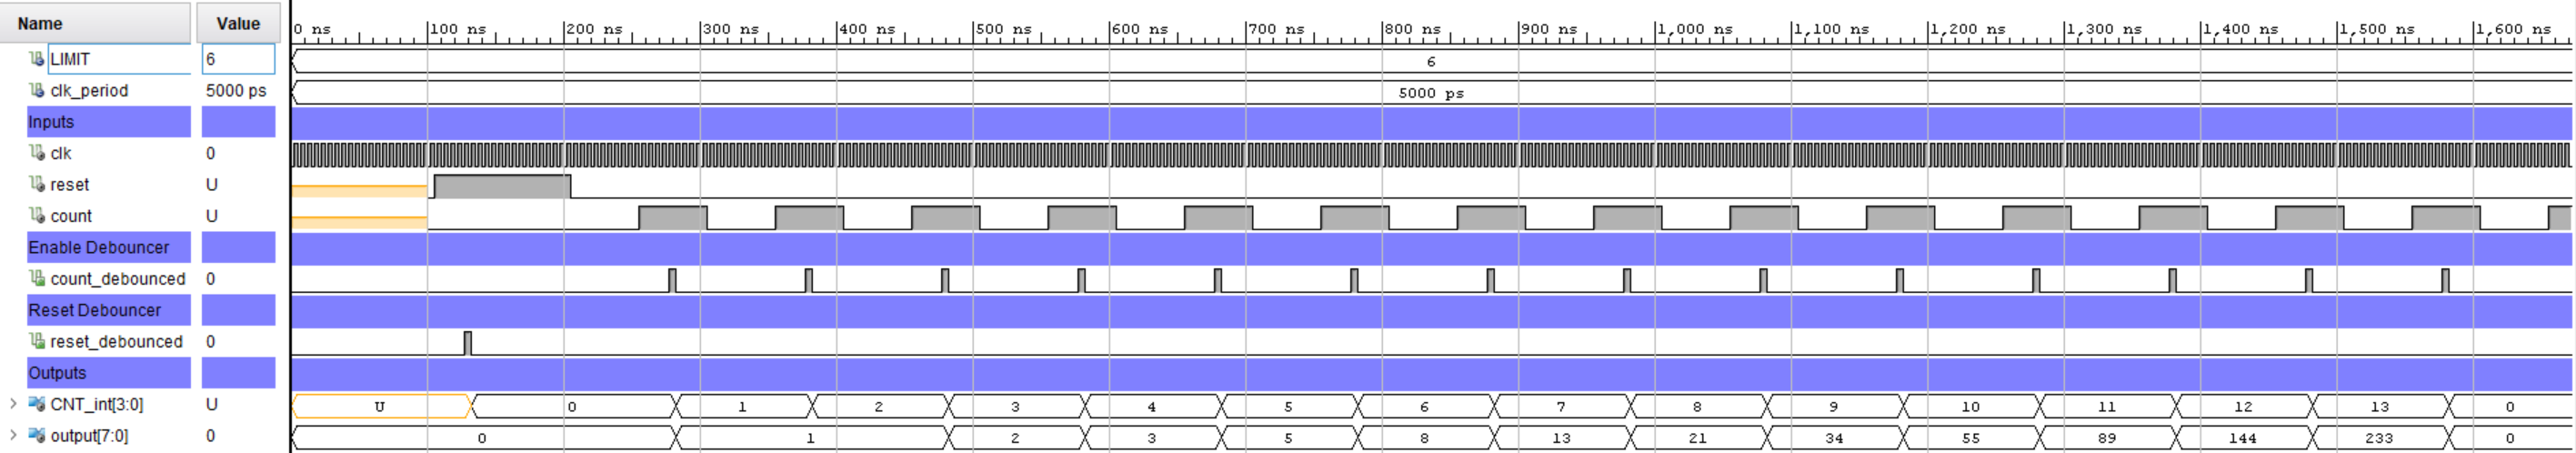
\includegraphics[width=\columnwidth]{Reports/Lab1/Waveforms/01_entire-sequence.png}
\end{figure}
The above waveform screenshot shows the entire sequence from time 0 to output 1 after a roll-over. This waveform is intended to verify that the overall output is correct.

\subsubsection*{Test 1, Waveform 1 - Initial reset and counting}
\begin{figure}[H]
    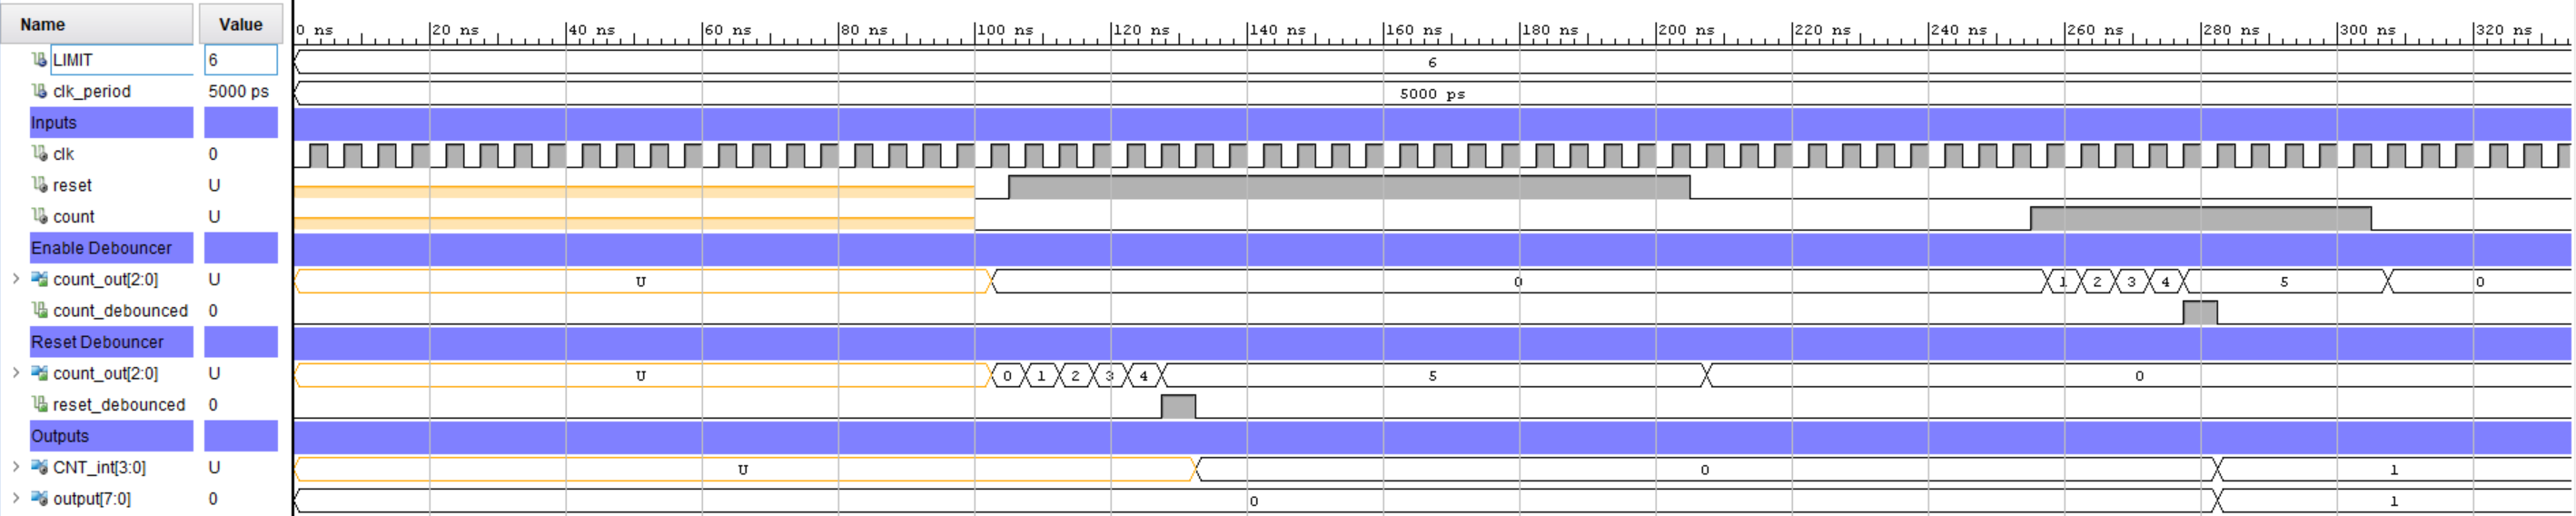
\includegraphics[width=\columnwidth]{Reports/Lab1/Waveforms/02_initial-reset-and-counting.png}
\end{figure}
The above waveform shows the initial global reset, verifying a successful activation of both the `reset' and `count' debouncers and a successful reset and increment of the overall circuit. 

\subsubsection*{Test 1, Waveform 2 - Counting up}
\begin{figure}[H]
    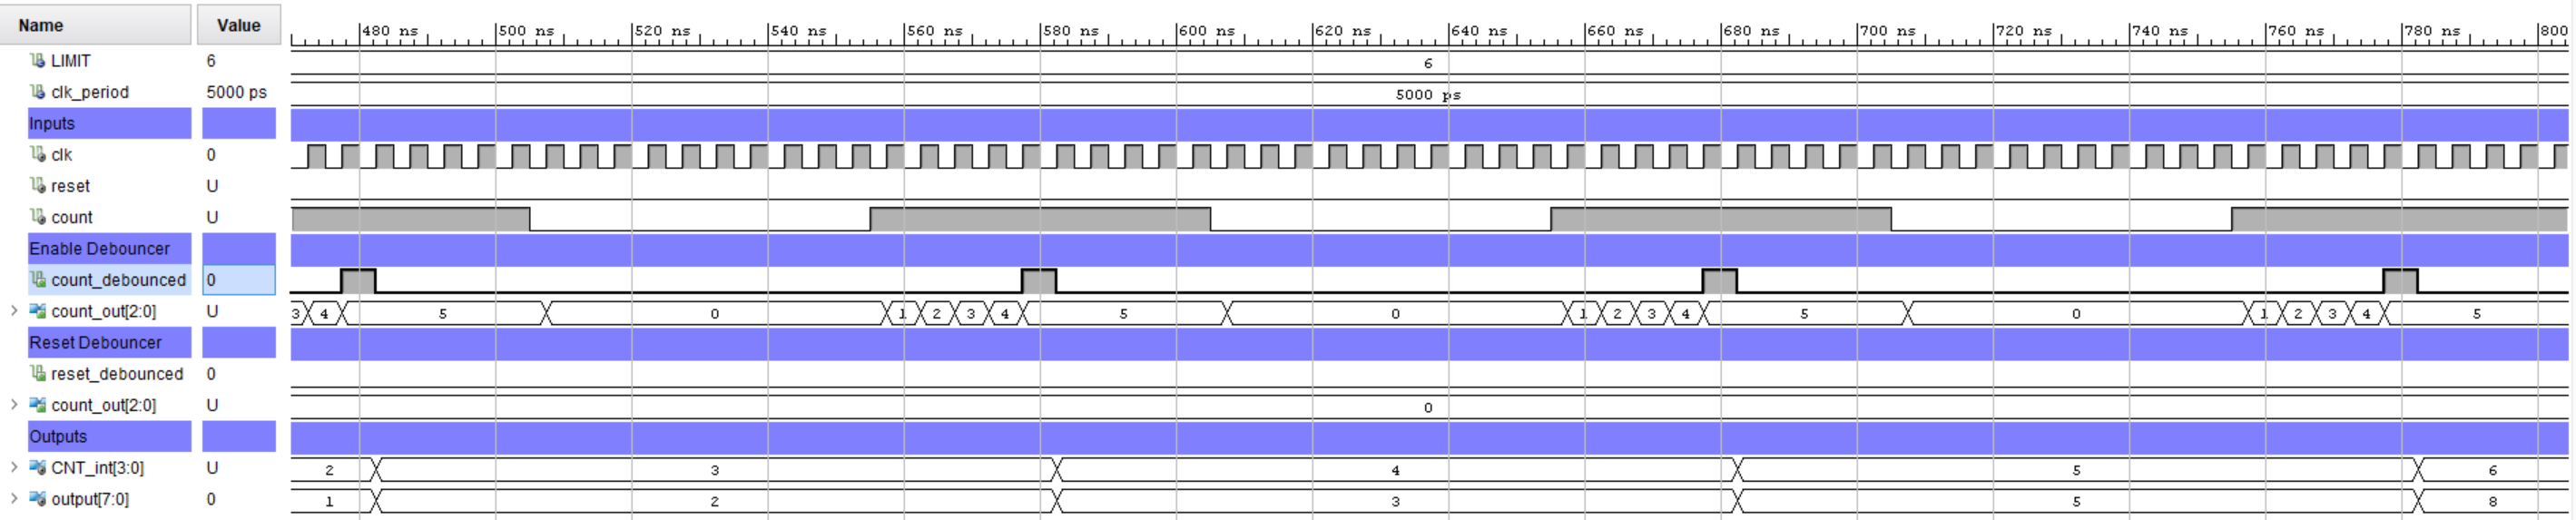
\includegraphics[width=\columnwidth]{Reports/Lab1/Waveforms/03_counting-up.png}
\end{figure}
This waveform (a continuation of Test 1, Waveform 1) verifies that the debouncer is activating and the counter increments as designed, the Fibonacci sequence is shown (1,2,3,5,8).

\subsubsection*{Test 1, Waveform 3 - Roll-over and count up}
\begin{figure}[H]
    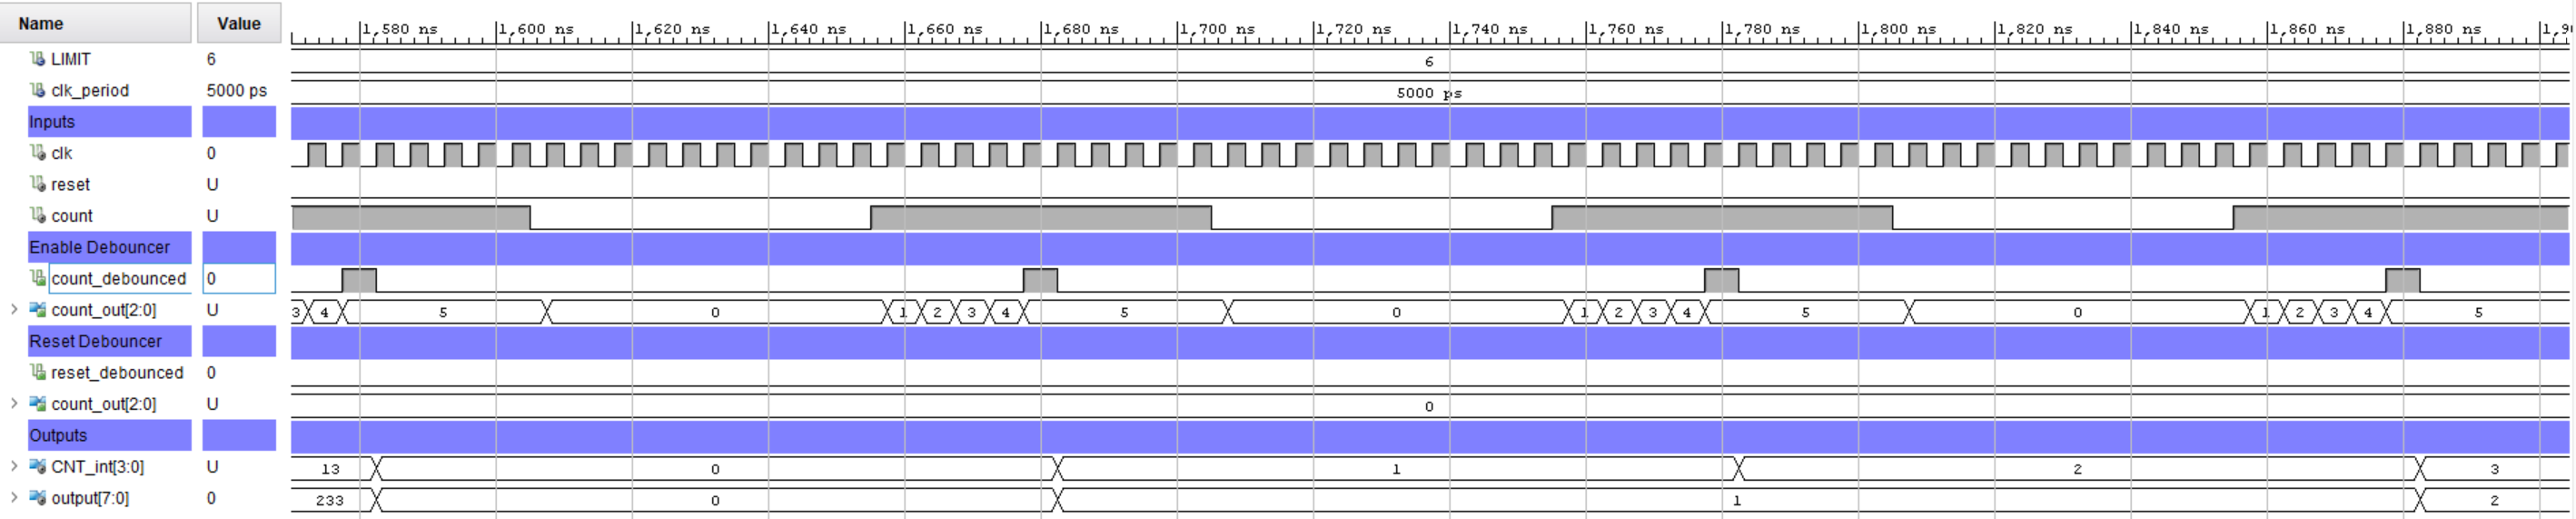
\includegraphics[width=\columnwidth]{Reports/Lab1/Waveforms/04_roll-over-and-count.png}
\end{figure}
This waveform verifies that the maximum Fibonacci sequence value is reached, and the sequence rolls over to 0 without a reset signal being generated by the user and can resume counting up.

\subsubsection*{Test 2 - Quick reset pulse}
\begin{figure}[H]
    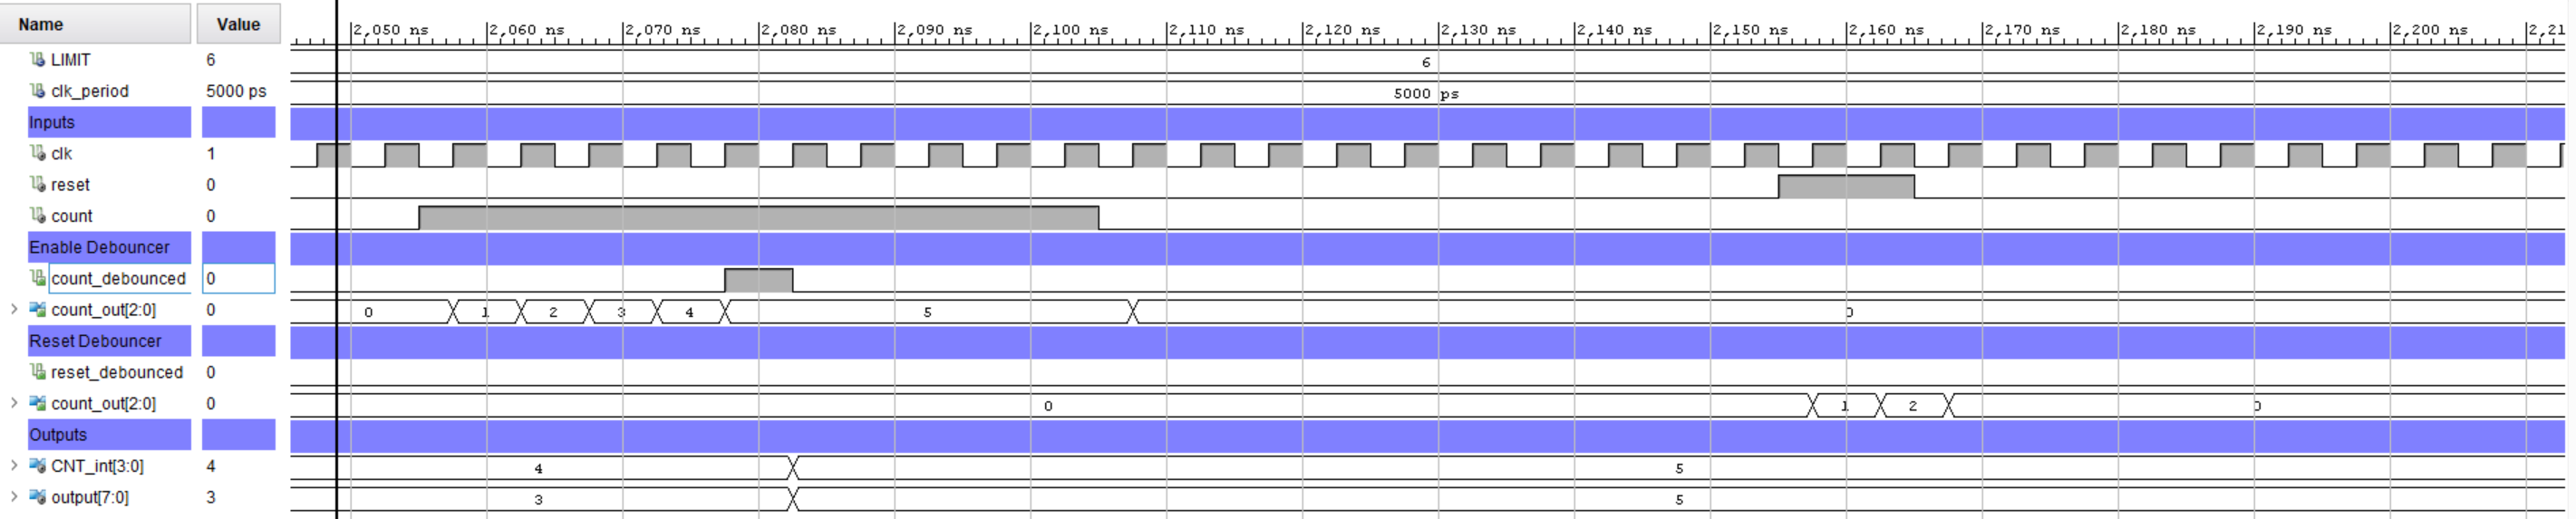
\includegraphics[width=\columnwidth]{Reports/Lab1/Waveforms/05_quick-reset-pulse.png}
\end{figure}
This waveform verifies that the debouncer is functioning as intended by showing the parameterizable counter on board the debouncer incrementing when the reset signal is high but resetting as soon as it goes low before the `LIMIT' is reached, thus invalidating the reset input.

\subsubsection*{Test 3 - Longer reset pulse}
\begin{figure}[H]
    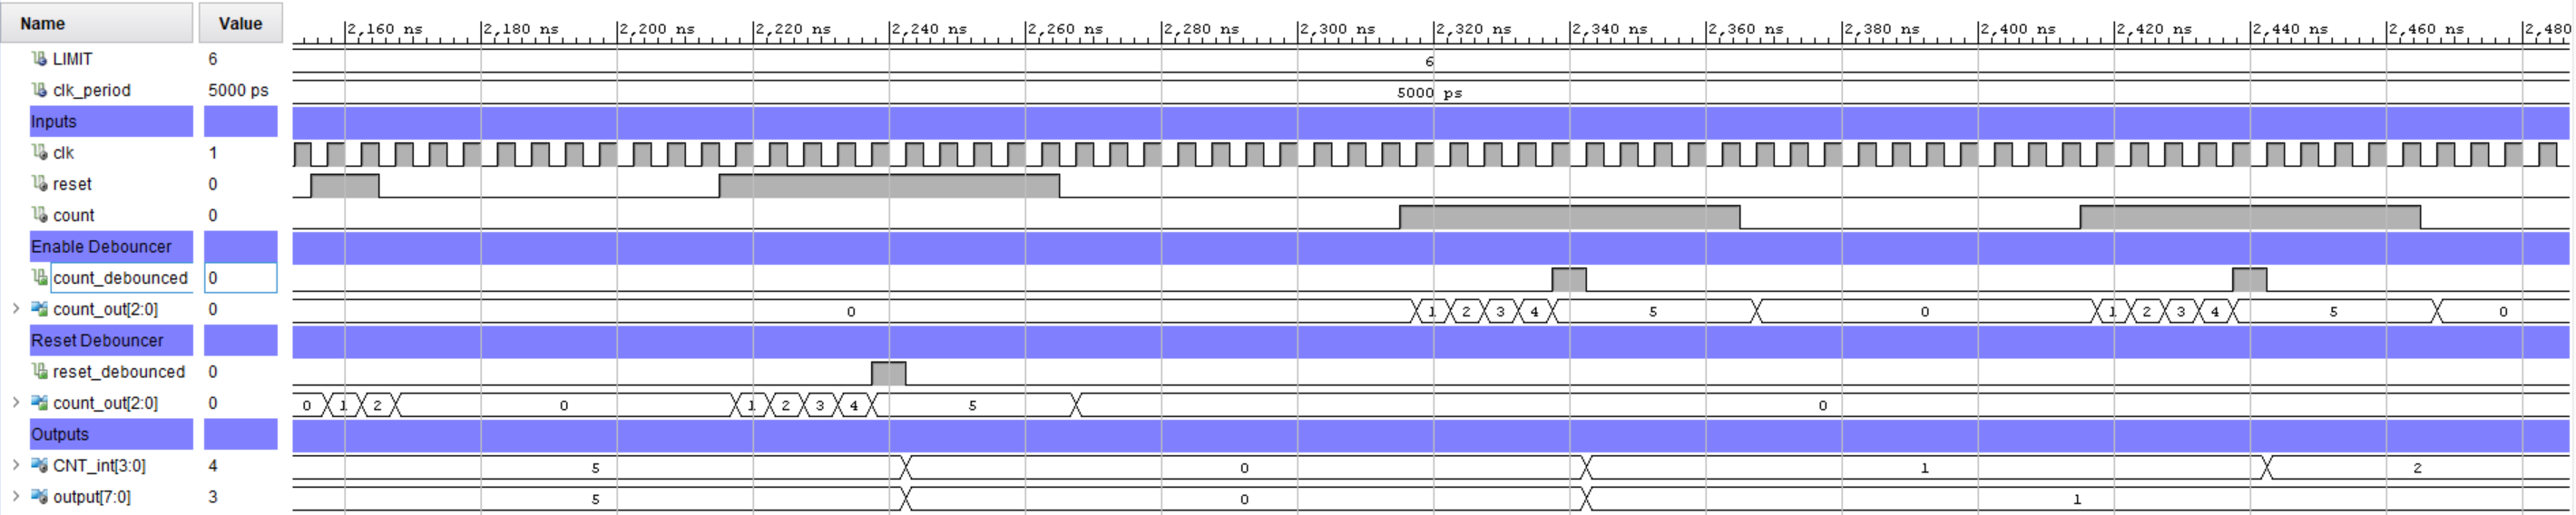
\includegraphics[width=\columnwidth]{Reports/Lab1/Waveforms/06_longer-reset-pulse.png}
\end{figure}

This waveform verifies that the debouncer successfully activates with a longer reset pulse of a valid clock duration. The counter in the debouncer increments with each clock cycle while the reset is high, and outputs a high debounced output once `LIMIT' is reached.

\subsubsection*{Test 4 - Resume after mid-operation reset}
\begin{figure}[H]
    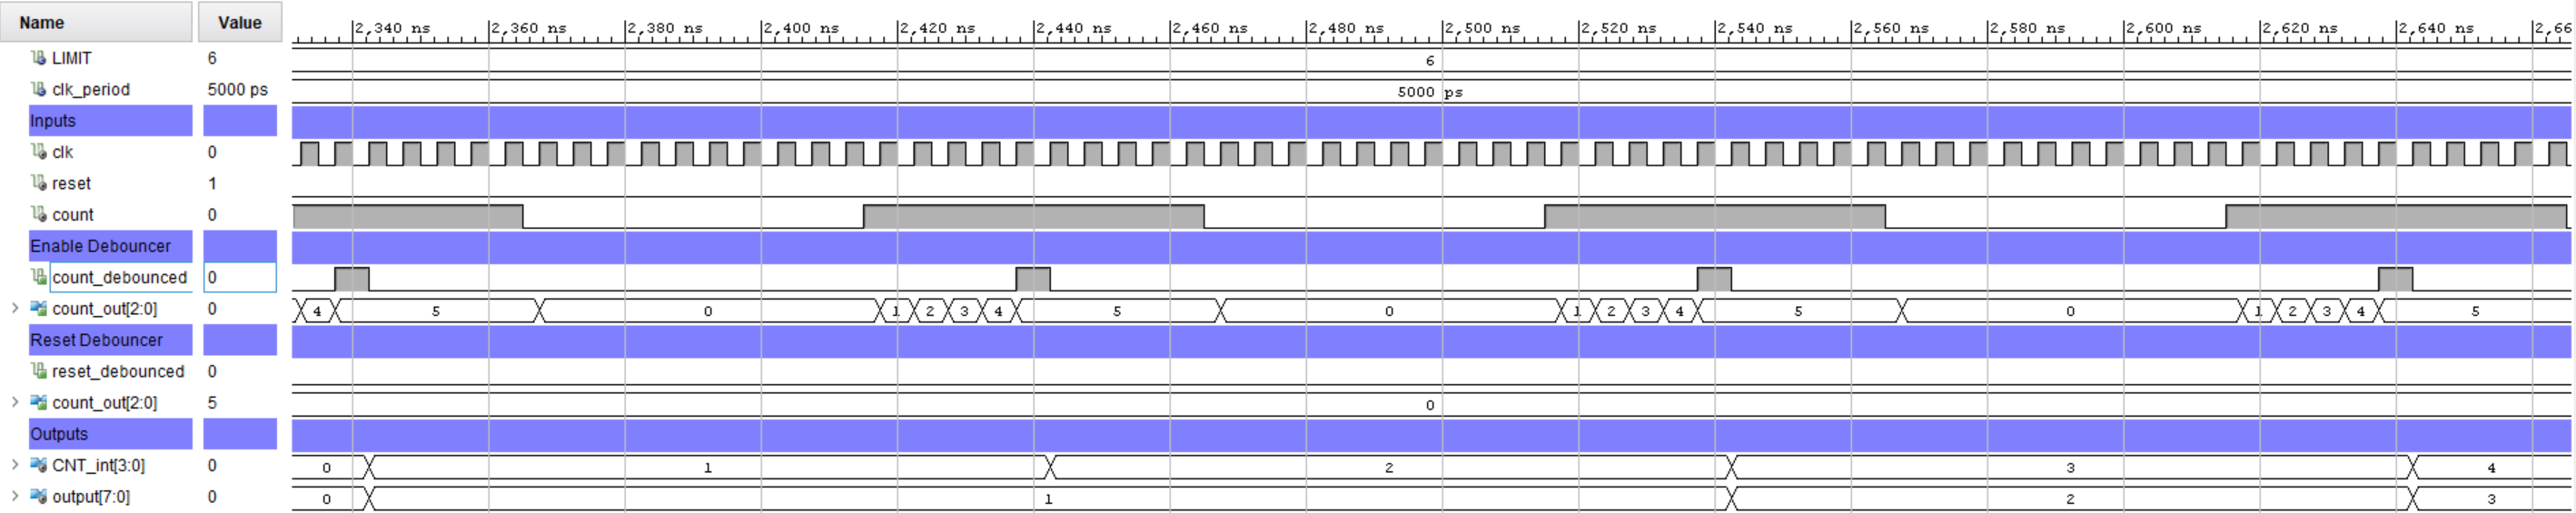
\includegraphics[width=\columnwidth]{Reports/Lab1/Waveforms/07_resume-after-mid-operation-reset.png}
\end{figure}
This waveform verifies that the circuit successfully resumes counting after a mid-operation reset following Test 3.

\subsubsection*{Test 6 - Holding reset and count}
\begin{figure}[H]
    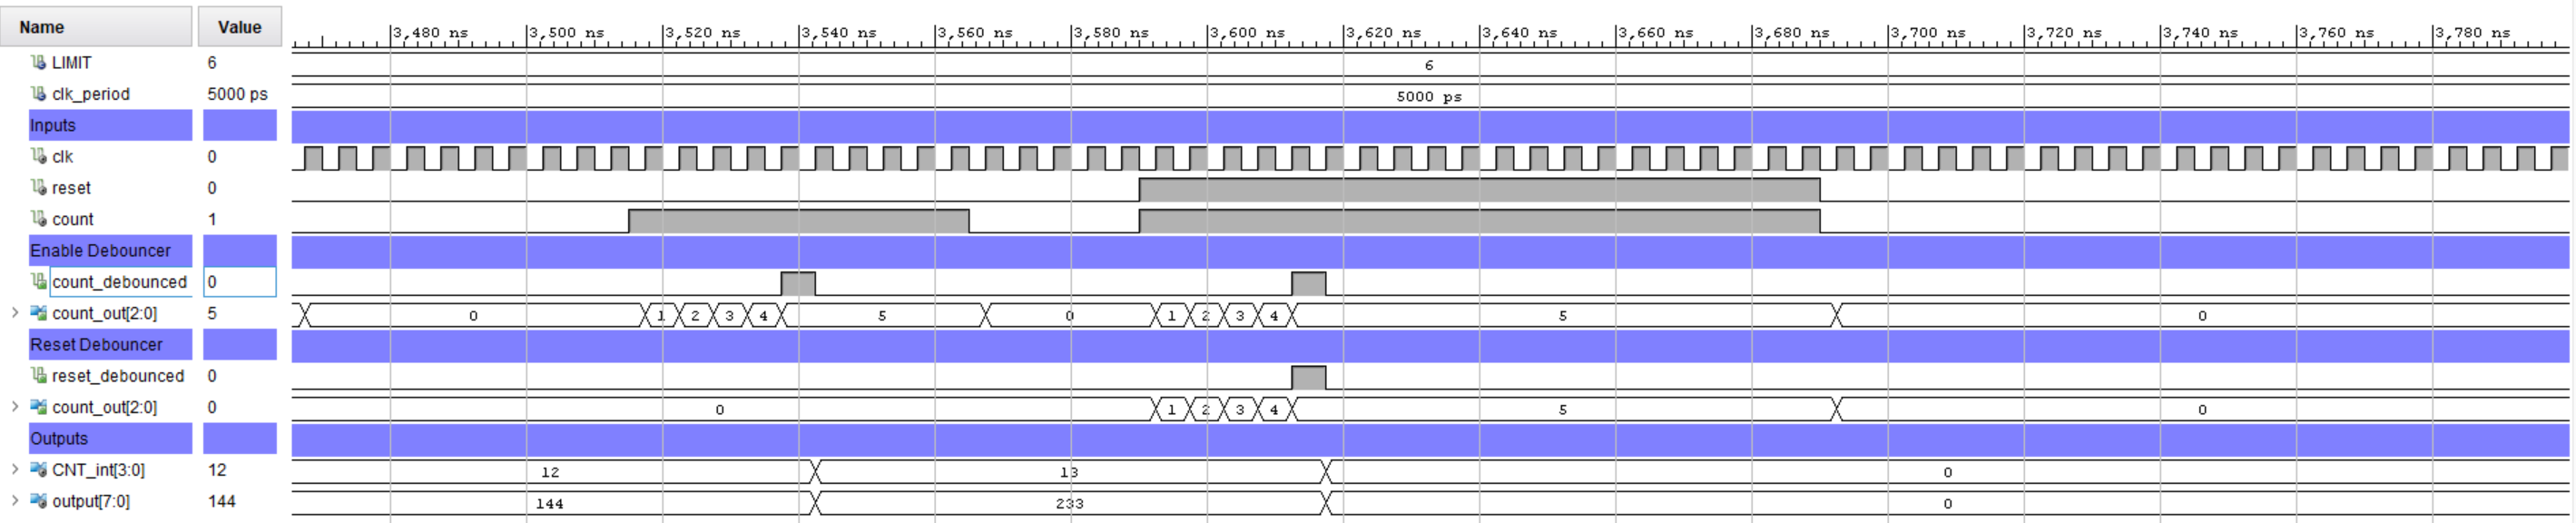
\includegraphics[width=\columnwidth]{Reports/Lab1/Waveforms/08_holding-reset-and-count.png}
\end{figure}




\section*{Circuit Analysis and Synthesis}

\subsection*{RTL Componenet Statistics}
\inputminted[firstline=65,lastline=76]{text}{../../Lab1/Lab1.runs/synth_1/fibonacci_8bit_sequence.vds}

\subsection*{RTL Hierarchical Component Statistics}
\inputminted[firstline=83,lastline=107]{text}{../../Lab1/Lab1.runs/synth_1/fibonacci_8bit_sequence.vds}

From the circuit design phase of this lab, we developed the `LIMIT' parameter to have a size of 50,000,000 so that when running on a 1MHz FPGA, inputs lasting less than 0.5 seconds would be ignored. As the `parameterizable\_counter' entity on board each debouncer will have to count up to the `LIMIT' parameter, the entity will need to be 26 bits in size ($\log_2(50,000,000)=25.58\approx26$). So it makes sense that the counter has been synthesised as 26 bits in size.



\subsection*{Schematics}


\subsubsection*{RTL Top Level (ROM Expanded)}
\begin{figure}[H]
    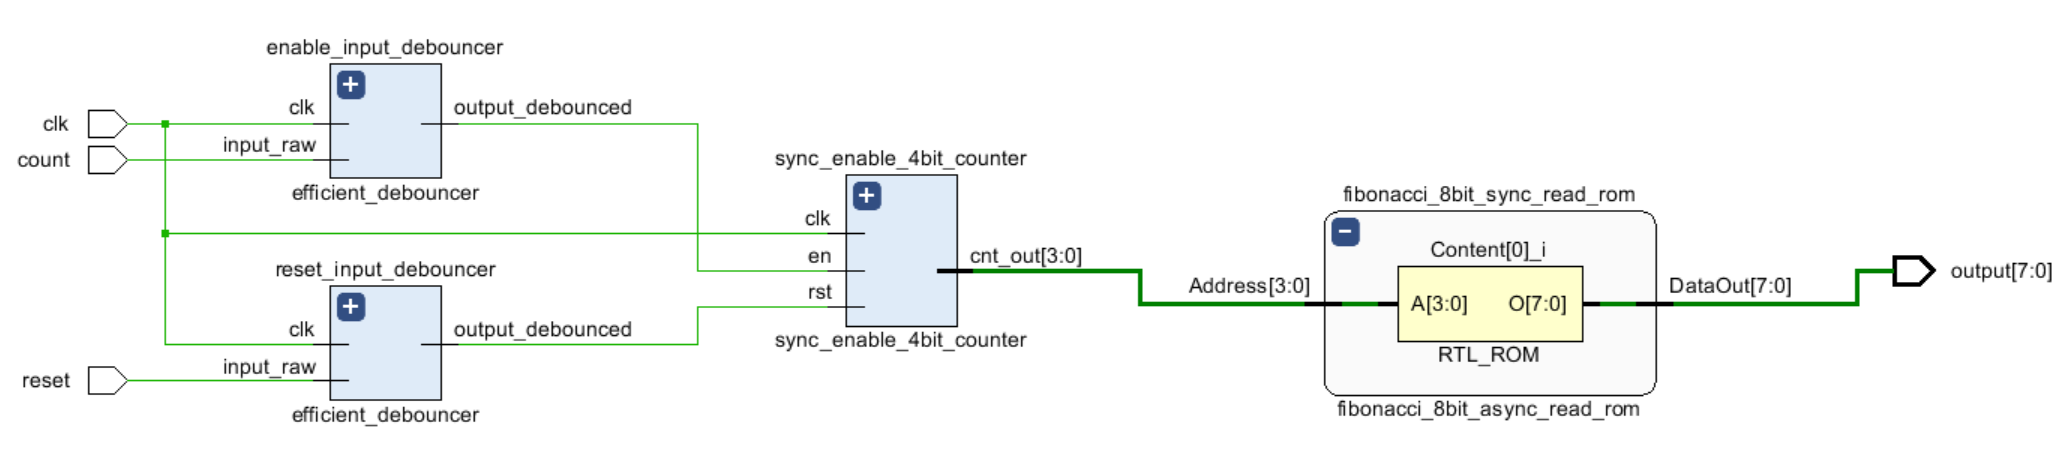
\includegraphics[width=\columnwidth]{Reports/Lab1/Schematics/01_rtl-tl-rom-expanded.png}
\end{figure}
As designed, there's a debouncer each for the `reset' and `count' raw input signals. These debounced signals are what control the 4-bit counter which accesses the Fibonacci ROM.



\subsubsection*{RTL Debouncer}
\begin{figure}[H]
    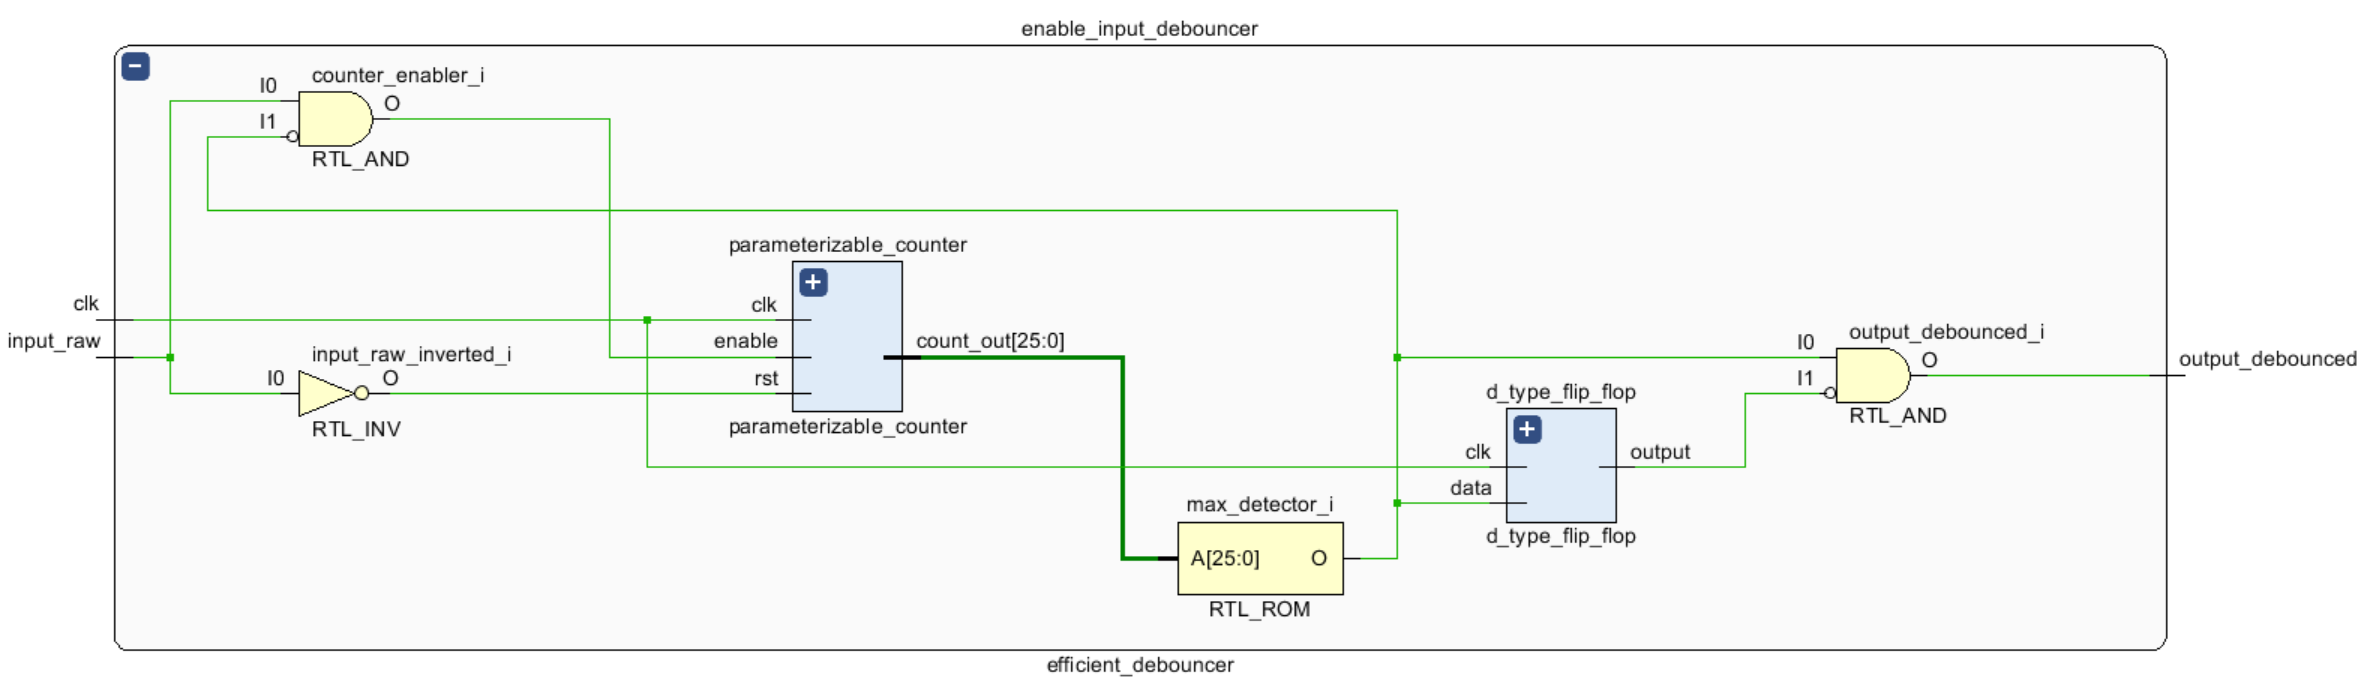
\includegraphics[width=\columnwidth]{Reports/Lab1/Schematics/02_rtl-debouncer.png}
\end{figure}
The clock signal is input along with the raw input for debouncing. Whilst the raw input is high and the max value (`LIMIT') hasn't been reached, the counter will increment. Once the `LIMIT' has been reached, `enable' goes low, which stops the counter from incrementing. The counter is reset once the raw input goes low.

When the `LIMIT' has been reached, a high signal output from the `max\_detector' is stored in the d-type flip flop. The same output is compared with an AND gate with an inverted output from the d-type flip flop, this is to ensure the debouncer doesn't activate for more than one clock cycle.

\subsubsection*{Synthesis Top Level (ROM Expanded)}
\begin{figure}[H]
    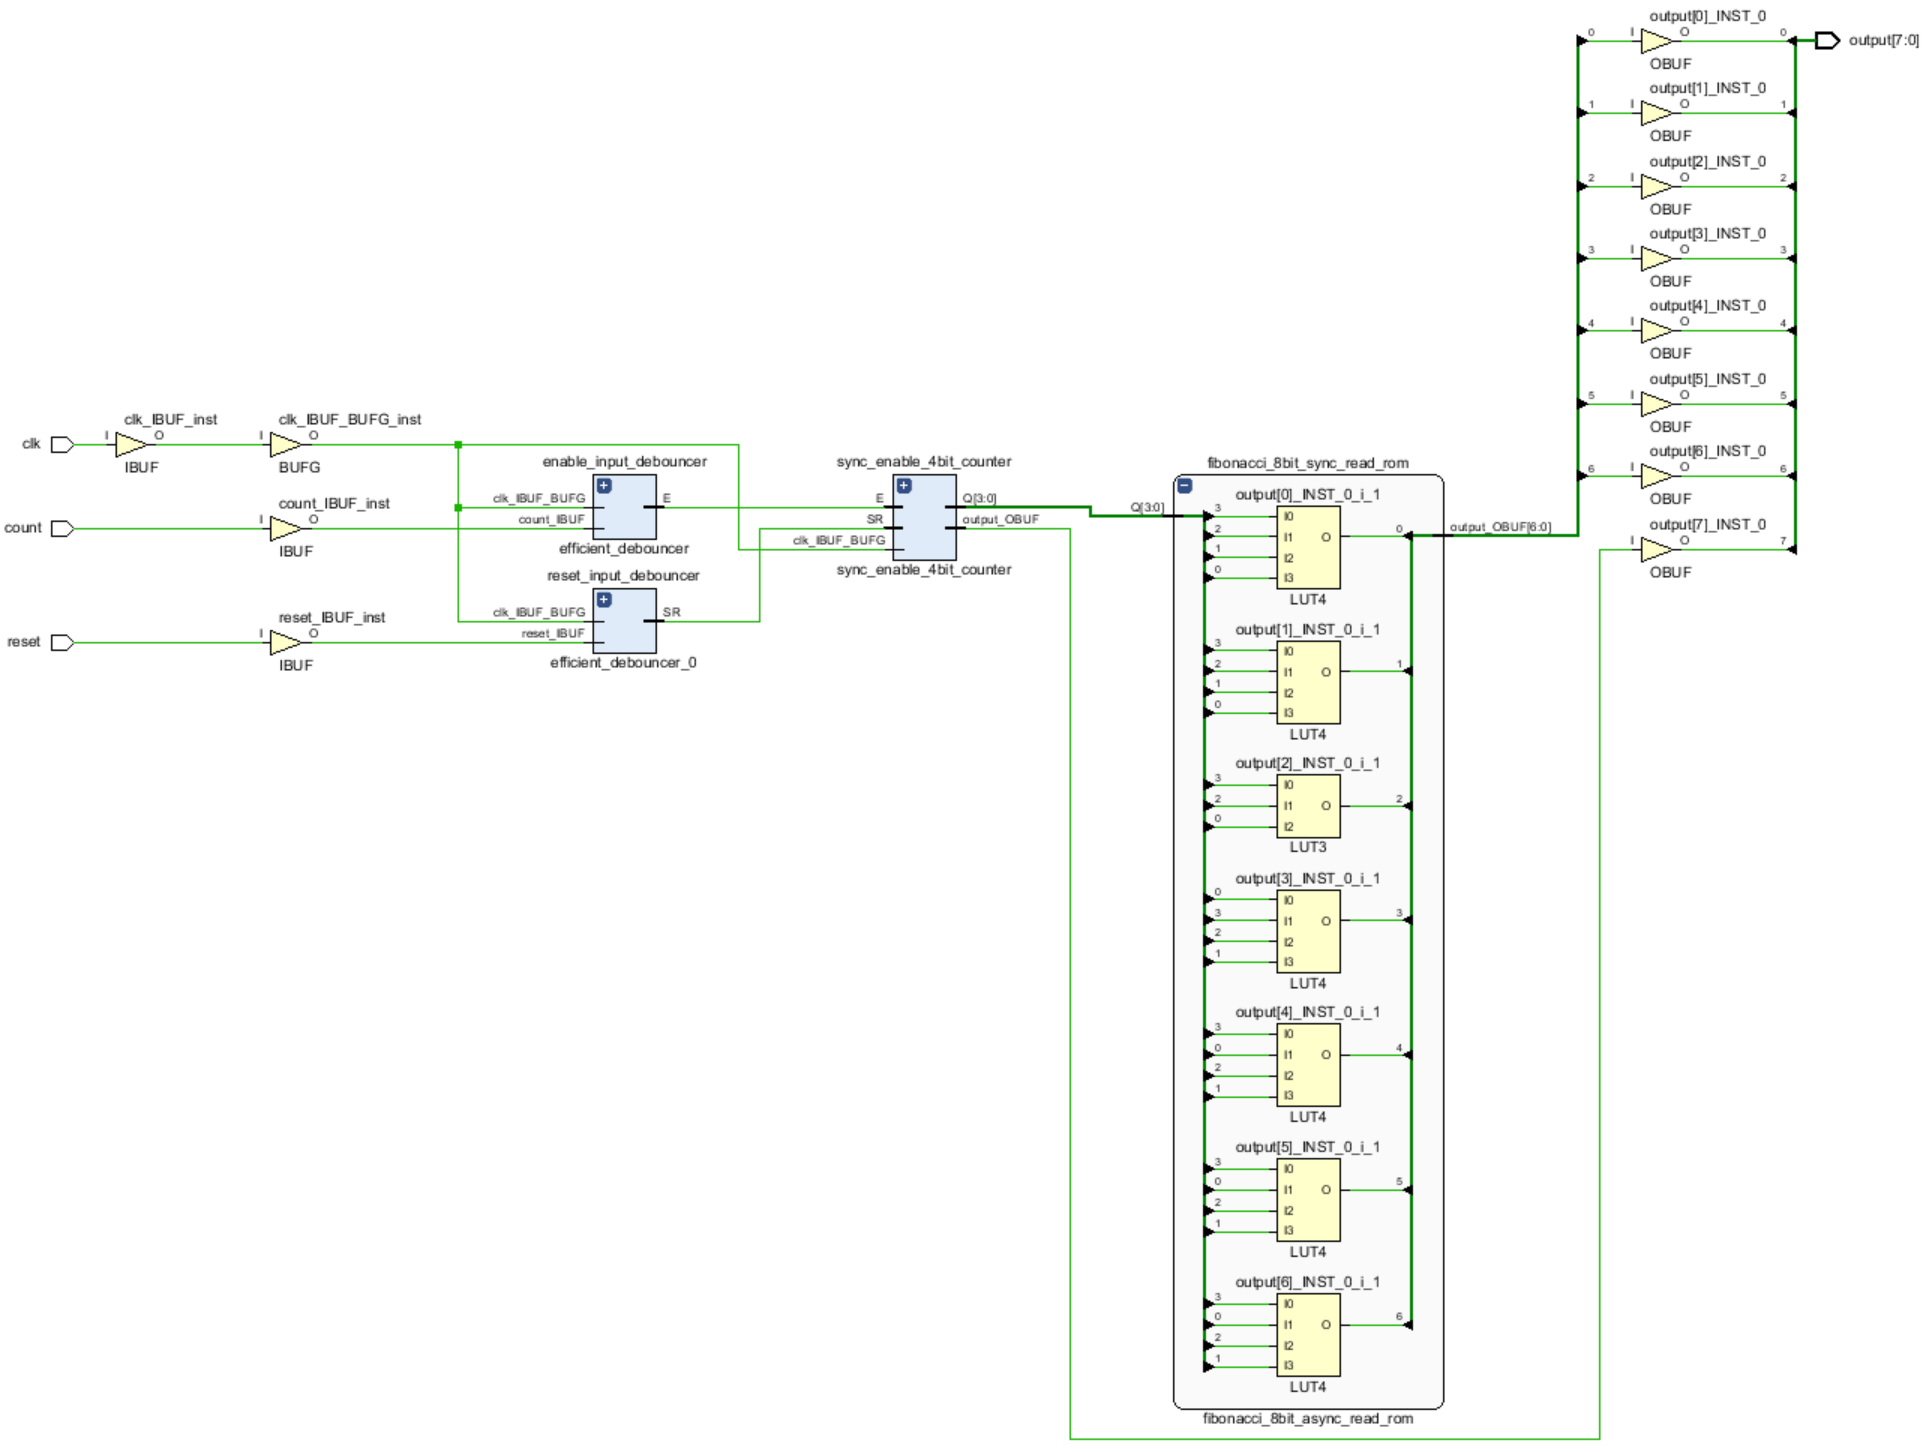
\includegraphics[width=\columnwidth]{Reports/Lab1/Schematics/03_synth-tl-rom-expanded.png}
\end{figure}
There are input buffers for each input pin. The clock pin has an additional buffer (BUFG) which is used to distribute high fan-out clock signals. The ROM is synthesised as an array of look-up tables. And finally, each signal in the output bus has an output buffer.

\end{document}
